\section{Backend filtering strategies}

Up until this point in the thesis, we have focused mostly on the marking phase of garbage collection. While this is understandable given that, in our modular collection scheme, the implementation--and thus behavior--of the filtering phase is left to the Irmin backends, this chapter will give a few insights to help the implementation of \texttt{filter} in the non-trivial case of pack-file backends.

\subsection{Pack-file backends}

As mentioned in the introduction, Irmin currently supports several storage backends: \texttt{irmin-mem}, which stores objects in a hashtable in memory; \texttt{irmin-fs}, which persists serialized objects on a POSIX filesystem; \texttt{irmin-git}, which provides a layer of compatibility with Git repositories; and \texttt{irmin-pack}, which persists serialized objects in a single large file similar to a block device.

Since implementing the \texttt{filter} operation is trivial in the case of \texttt{irmin-mem}, \texttt{irmin-fs} and \texttt{irmin-git}, we will exclusively focus on the more complex \texttt{irmin-pack} backend, which was introduced in Irmin 2~\cite{irmin-2-blog} as a way to provide fast and non-blocking access for Irmin objects while reducing the disk footprint of large stores--for instance, the disk usage of Tezos nodes was reduced tenfold after switching from an LMDB-based backend to \texttt{irmin-pack}.

\bigskip
In essence, an instance of \texttt{pack} is a combination of the following elements:
\begin{itemize}
  \item
        The \emph{pack}, shown in \cref{fig:pack}. It is a single append-only file stored on disk which contains a binary encoding--as well as a few bytes of header--of all the objects in the backend. In the algorithms to follow, we will interact with the pack using the following signature:

        \begin{minted}{ocaml}
val read : t -> off:int64 -> bytes -> int
(** [find t ~off b] fills the buffer [b] with the contents of [t] between the
    offsets [off] and [off + size(b)]. Returns the number of bytes read. *)

val offset : t -> int64          (** Returns the current end offset of [t]. *)
val append : t -> string -> unit (** Appends bytes to the end of [t]. *)
val clear : t -> unit            (** Clears the contents of [t]. *)
  \end{minted}
        \vspace{-1em}

  \item
        The \emph{dict}, which is also a single append-only file stored on disk, but is used solely to de-duplicate the names of paths when storing nodes. For the sake of simplicity, we will ignore it in the algorithms to follow--it can be handled like the pack.

  \item
        The \emph{index}, available as a standalone package at~\cite{index-github}. It is a multi-level index persisted on disk, and is used here to associate the hashes of objects with the offset at which they are encoded in the pack. For the sake of brevity, we won't get into details about its implementation; in what follows, we will simply treat it as a black-box with the following signature:

        \begin{minted}{ocaml}
val clear : t -> unit         (** [clear t] removes all the bindings in [t]. *)
val find : t -> key -> value  (** [find t k] is the binding of [k] in [t]. *)
val mem : t -> key -> bool.   (** [mem t k] is [true] iff. [k] is bound in [t]. *)

val replace : t -> key -> value -> unit
(** [replace t k v] binds [k] to [v] in [t], replacing any existing binding of [k]. *)

val iter : (key -> value -> unit) -> t -> unit
(** [iter f t] iterates [f] over the bindings in [t]. *)
  \end{minted}
\end{itemize}

\begin{figure}[ht]
  \caption{Layout of the \texttt{pack} in a pack-file backend.}
  \label{fig:pack}

  \centering
  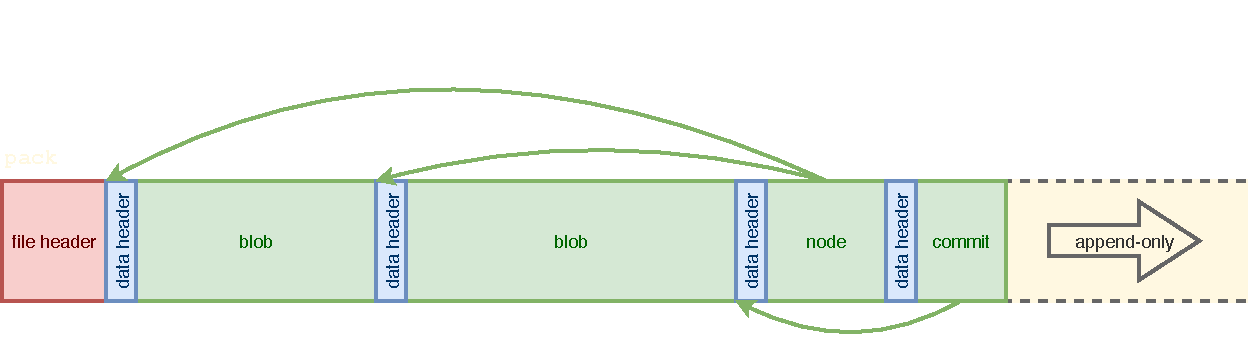
\includegraphics[trim={0 1em 0 3.8em},clip,width=0.85\textwidth]{images/pack.pdf}
\end{figure}


With this in mind, \cref{app:pack-backend} gives a simplified implementation of the \texttt{CONTENT\_ADDRESSABLE\_STORE} interface for a pack-file backend.

\subsection{Copying strategy for pack-file backends}

To implement the \texttt{filter} function in the backend above, I first drew inspiration from the idea of \emph{semispace copying collection} introduced in~\cite{feni69}. In short, copying collectors divide the heap into two equally sized \emph{semispaces}--only one of which is active at any given time. New objects are allocated at the end of the active semispace; and collection can simply be implemented by copying all the marked objects from the active semispace to the other, leaving the unreachable objects behind. The roles of the two semispaces are then switched atomically, and the previously active semispace is reclaimed as a whole--generally by simply resetting its end pointer to the beginning.

Transposing this idea to Irmin, we get the implementation from \cref{app:pack-copying}. It uses two sets of \texttt{Pack.t} and \texttt{Index.t}--one for each semispace. This is equivalent to splitting the pack and the index in two parts, but has the significant advantage that it doesn't require modifying the \texttt{Pack} and \texttt{Index} modules in any way. When \texttt{filter} is called, the backend iterates over all the entries in the current index--i.e.~over all the stored objects--and copies only those which pass the predicate \(p\) to the new index and pack.

This strategy has several advantages: first of all, it is straightforward enough that a bug-free implementation can realistically be produced even when dealing with concurrency or with single-writer multiple-reader parallelism. As mentioned above, it also doesn't require cluttering the behavior of \texttt{Index} and \texttt{Pack} with unrelated concerns. That said, it also has several drawbacks: first, its runtime is proportional to the number--more accurately to the total size--of elements stored in the backend, so calls to \texttt{filter} can quickly get expensive even when there are just a few objects to reclaim. Also, during a call to \texttt{filter}, the disk footprint of the backend can temporarily grow to twice its regular size--which might become a problem for large stores.

\bigskip
A few words about concurrency: as mentioned in the previous chapter on \emph{Concurrent garbage collection}, the responsibility of dealing with concurrency when \texttt{filter} is called is left to the backends. In the implementation above, this is achieved by several means: first, the \texttt{filter} function is wrapped into an Lwt mutex to ensure that it cannot be called while previous calls are still running. As for concurrent calls to \texttt{set} and \texttt{filter}, remember that provides single-threaded cooperative multitasking: we are therefore guaranteed that multiple instructions will execute atomically as long as we don't yield back to the Lwt scheduler between them. In the implementation from \cref{app:pack-copying}, notice that the instructions between lines 85 and 102 never yield back to the scheduler, so the semispace copying is effectively atomic.

While this is generally acceptable, it might become problematic for larger stores--where blocking for the entire duration of the copying process would introduce noticeable mutator pauses. In this case, a solution would be to yield \emph{during} the iteration over \texttt{current\_index}; but we would need a way to make sure that concurrent calls to \texttt{set} don't interfere with the copy. While we could hijack calls to \texttt{set} so that they directly write to the other semispace when \texttt{filter} is running, it is generally not desirable as it might alter the relative ordering of objects in the pack--which we rely on for the generational garbage collection algorithm described above. A better option is to allow calls to \texttt{set} to append to the \texttt{current\_pack} as usual, but to record the end offset \(end\) of the \texttt{current\_pack} at the beginning of the call to \texttt{filter}, and then--during the copying phase--to copy only the objects which pass \(p\) \emph{and} with an offset \(off < end\). Finally, once all such objects are copied, we would block only for the time it takes to copy all the objects with an offset \(off' >= end\)--in other words the objects which were added concurrently.

\subsection{Lazy strategy for pack-file backends}

As mentioned above, the copying implementation of \texttt{filter} has several issues: is that it has a runtime proportional to the number of objects in the store, so it is expensive for large stores even when there are only a few objects to reclaim; and it potentially doubles the disk footprint of the backend for the duration of the call to \texttt{filter}. What follows is an alternative strategy--inspired by the classical mark-and-sweep algorithm--which tries to solve this problem by using switching some of the burden to \texttt{set}.

\bigskip
Precisely, instead of copying all the black objects to another semispace when calling \texttt{filter}, this strategy lazily reclaims the space used by white objects by adding it to a \emph{free list}; such that when \texttt{set} is later called, the backend first tries to allocate new objects into the previously reclaimed space, and falls back to appending at the end of the \texttt{pack} if there is not enough space.

While this strategy has the clear advantage of reducing the runtime and disk overhead of calls to \texttt{filter} dramatically, it comes with two significant trade-offs: first, it can clearly not be used in combination with the generational garbage collection algorithm described in the previous chapter, since the offsets of objects no longer correspond to the time they were added to the pack. More importantly, calls to \texttt{set} are no longer constant-time, but instead have a worst-case runtime of \(O(l)\) with \(l\) the current number of elements in the free list. Although the overhead is usually negligible at first, it might become problematic in the case of \emph{fragmentation}--i.e.~when the free list starts to contain many \((offset, length)\) pairs whose \(length\) is too small to allocate most objects.

How fragmentation evolves over the lifespan of the backend depends mostly on the strategy being used to choose pairs from the free list when allocating an object of size \(length'\): the naive strategy, called \emph{first-fits}, picks the first \((offset, length)\) pair in the list such that \(length >= length'\), removes it from the list, and ``splits'' the corresponding area of memory by putting back \((offset + length', length - length')\) into the list. It should be clear that, when using this strategy, the free-list will become ``polluted'' over time with pairs such that \(length - length'\) is smaller than the size of most objects, leading to a lot a fragmentation. Among the better strategies, \emph{segregated-fits}~\cite{comf64} works by partitioning the set of possible object sizes into arbitrary \emph{size classes}, and uses a free list for each size class instead of a single one. Then, when \texttt{set} tries to find space for an object of size \(length'\), it only has to go through a single free list.

Unfortunately, even if allocation strategies like segregated-fits generally help reduce fragmentation, it can never be fully avoided when free lists are used; and the problem only grows with the number of calls to \texttt{filter} and \texttt{set}. To mitigate the issue, a good compromise is to use the lazy version of \texttt{filter} whenever possible, but to fall back to copying collection whenever fragmentation becomes too important--as a way to compact the ``holes'' in the pack. \cref{app:pack-lazy} provides an implementation of this hybrid strategy. It uses first-fits allocation for the sake of clarity, but can easily be extended to segregated-fits allocation. To keep track of fragmentation, it measures both the number of already reclaimed objects and the ratio between the size of black objects in the pack and the total size of the pack; and it chooses to run the \emph{compacting} version of \texttt{filter} whenever one of these metrics reach a predefined threshold.

Another cause of concern with such a strategy is that writing to the pack-file at random offsets instead of only at its end could have a noticeable runtime overhead. To determine whether this could become a problem, I benchmarked the performance of disk operations on an SSD when using different access patterns and different file modes. The results are available in \cref{app:disk-access}--in short, although there is a noticeable overhead to calling \texttt{seek} then \texttt{write} sequentially when writing at random offsets in a file, it is actually coming from the fact that we are making two system calls rather than from the performance of the disk itself, which can be solved by using the combined \texttt{pwrite} system call instead.

\subsection{Avoiding fragmentation by using interval trees}

Finally, I experimented with ways to significantly reduce the possibility of fragmentation in the previous scheme--so that calls to \texttt{compact\_filter} would no longer be needed. A key insight is to realize that fragmentation can occur for two distinct reasons: either an isolated chunk of the pack was reclaimed, but it is too small for any new object to be allocated in its place; or a large enough portion of the pack is reclaimable, but it is split into many contiguous \((offset, length)\) pairs in the free list--each of them too small to receive a new object. While the first reason is unavoidable, notice that the second one is purely a consequence of the data structure being used: what if, instead of using a free list, we used something more suited to the storage of intervals?

Interestingly enough, there are very few attempts at using structures other than linked lists for allocation in garbage collection literature. This is most likely due to the fact that allocators of memory-managed programming languages are incredibly performance-sensitive, and so the few extra CPU cycles needed to use a more complex data structure are generally prohibitive. In the case of pack-file backends for Irmin, however, this becomes a much more reasonable trade-off--not least because \texttt{set} generally writes to the disk, so the overhead of a few more CPU cycles becomes negligible.

\bigskip
For this experiment, I settled on using an OCaml implementation of Discrete Interval Encoding Trees~\cite{erwig89} available at~\cite{diet-github}, whose abridged signature is given in \cref{app:diet-sig}. Concisely, this data structure uses a binary search tree to store sets of \emph{non-overlapping} discrete intervals. Note that this data structure is \emph{not} an interval tree, since the non-overlapping invariant means that adding \(\llbracket 1, 2 \rrbracket\) to the set \(\{\llbracket2, 3\rrbracket, \llbracket4, 5\rrbracket\}\) will give the set \(\{\llbracket1, 3]], \llbracket4, 5\rrbracket\}\). This would eliminate some fragmentation in free-list backends, since contiguous reclaimed intervals of the pack would be merged together. Let \(n\) be the number of non-overlapping intervals in the DIET. This implementation uses \(O(n)\) storage, and provides \texttt{cardinal} and \texttt{choose} in \(O(1)\) runtime, while \texttt{add} and \texttt{remove} are in \(O(\log{n})\) on average but \(O(n)\) in the worst case.

Given these operations, one can easily write \mintinline{ocaml}{extract : elt -> t -> (interval * t) option} in \(O(n)\), such that \mintinline{ocaml}{extract n t} tries to extract an interval of size \mintinline{ocaml}{n} from \mintinline{ocaml}{t}, and returns either \mintinline{ocaml}{Some (i, rest)} with \mintinline{ocaml}{rest = remove i t} or \mintinline{ocaml}{None} otherwise. It would then be trivial to replace the free list in the strategy above with a DIET which stores a single interval for every non-overlapping chunk of the pack which was previously reclaimed. The implementation of \texttt{filter} would call \texttt{add} every time it finds a white object to reclaim, leading to a \(O(r \log{r})\) runtime when there are \(r\) white objects in the graph--instead of \(O(r)\) when using a free-list. The implementation of \texttt{set} would then call \texttt{extract} with the size of the object to allocate, leading to the same \(O(l)\) runtime as with a free list--with \(l\) the number of intervals in the tree.

Summing up, replacing the free list with a DIET would reduce the fragmentation caused by the free list in the previous strategy at the cost of a \(\log{r}\) factor during calls to \texttt{filter}; which is reasonable given that \texttt{filter} will not be called frequently. To confirm the viability of the strategy, I benchmarked the runtime and storage overhead of DIET operations with a varying number of stored intervals--see \cref{app:diet-bench}. Notice that, even with \(10^4\) intervals in the structure, the runtime of all operations mostly stays an order of magnitude below that of a disk access; so the overhead of the DIET would be negligible.